\chapter{移动机器人的定位与导航}
\label{cha:chapter03}

定位与导航功能在机器人开发中占有重要地位。一般的,我们认为机器人的定位
导航功能包含环境地图构建、路径规划与运动控制以及自主避障等子任务。Tinker
机器人的定位导航系统基于ROS框架下的Navigation Stack实现,使用激光雷达、
里程计、深度相机等多传感器融合方法,能够完成实时地图构建、重定位、动态
环境下的避障即导航任务。


\section{SLAM方案的选择与性能分析}

Tinker最初使用的是建图与定位分开实现的方案。建图方面,我们使用
gmapping算法\cite{grisettiyz2005improving},
依赖2个北洋UTM-30LX单线激光雷达拼接定位(如图\ref{fig:utm30lx})。定位
方面,我们使用基于蒙特卡罗的
amcl算法\cite{fox2002kld},两个算法同时工作时的可视化信息如图\ref{fig:gmapping_amcl}。
amcl需要在地图已经给出的情况下进行定位,在
真实赛场上,比赛场景多数情况下是确定的,因此这套方案还基本可用,Tinker团队
会在开赛前对赛场进行扫描,将地图场景保存起来,之后比赛过程中单纯使用amcl
进行定位。后期随着团队成员对这套定位算法越来越熟悉,我们会将场景内可能出现
在单线雷达视野内的一切固定障碍的尺寸量下来,使用绘图软件对地图进行重建,然后
使用amcl进行定位,可以拿到更好的定位效果。

\begin{figure}
  \centering
  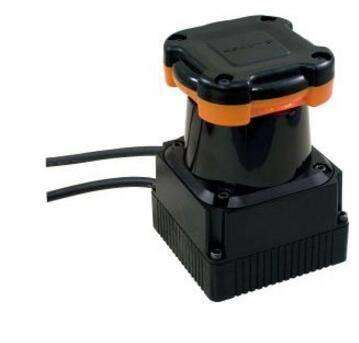
\includegraphics[width=300pt]{utm30lx.jpeg}
  \caption{北洋UTM-30LX单线激光雷达}
  \label{fig:utm30lx}
\end{figure}


\begin{figure}
  \centering
  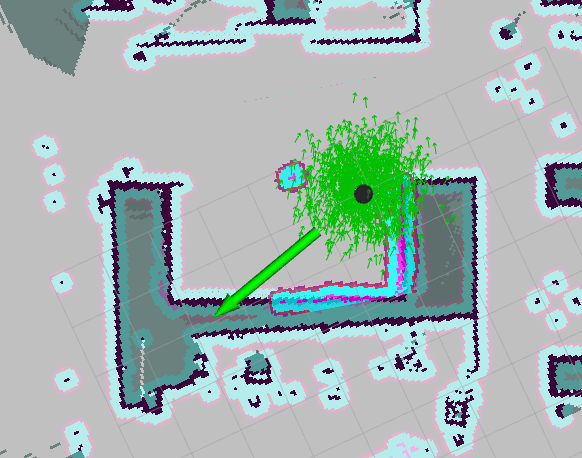
\includegraphics[width=300pt]{gmapping_amcl.png}
  \caption{Gmapping + Amcl可视化效果}
  \label{fig:gmapping_amcl}
\end{figure}

虽然上述方案在长时间内被证明是稳定可用的,但随着SLAM社区的不断发展,基于
粒子滤波的定位建图算法已经过时了,尤其是Google开源其自主开发的Cartographer
雷达建图定位算法\cite{hess2016real}之后,Tinker团队后期也将定位方案迁移为Cartographer+
ROS Navigation的模式,在更换建图定位算法之后,配合我们对Tinker硬件的二次
改版,我们也将原有的2个单线雷达减少为一个,变动之后定位数据减少,运算效率也
得到了提升。Cartographer的算法框架如图\ref{fig:cartographer}所示。

\begin{figure}[h] % use float package if you want it here
  \centering
  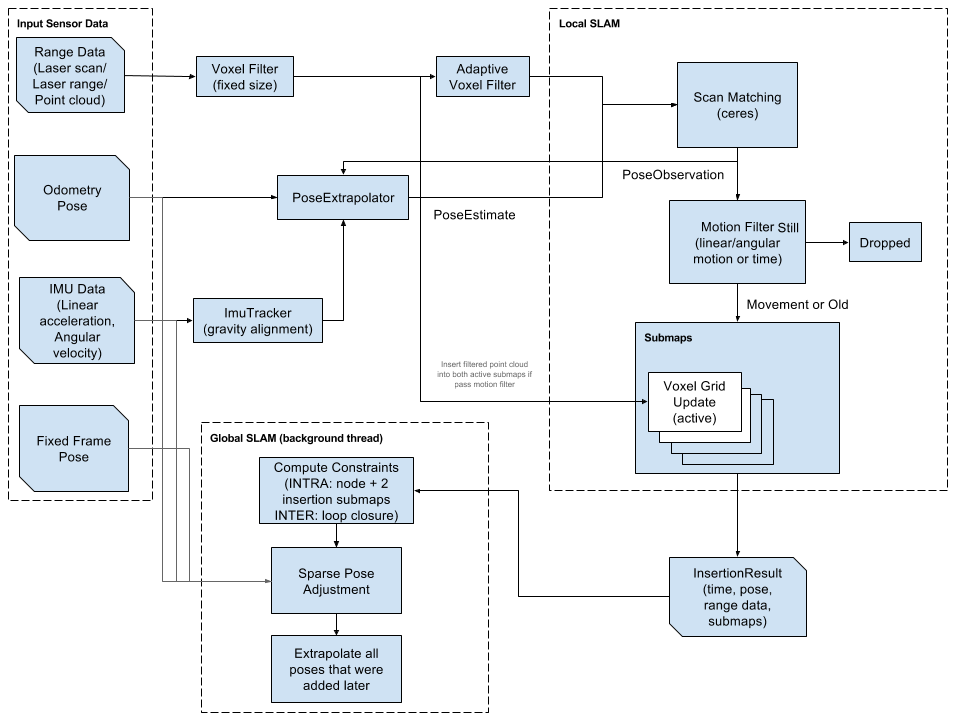
\includegraphics[width=300pt]{cartographer.png}
  \caption{Cartographer的算法框架}
  \label{fig:cartographer}
\end{figure}

除了基于单线激光雷达的各种定位建图算法外,笔者还尝试了一些基于特征点的视觉SLAM
方案,例如基于ORB特征点法的ORB-SLAM2(使用Kinect v2的RGB-D数据)\cite{mur2015orb},
ORB-SLAM2在室内环境中的可视化效果如图。。。所示。我们还测试了基于双目和IMU数据
融合的VINS-Fusion\cite{qin2018vins}算法,效果如图。。。所示,并且分析了两算法表现上的差异。

ORB-SLAM2的算法框架如图\ref{fig:orb_frame}所示,其获取到原始数据后,首先对



\begin{figure}[h] % use float package if you want it here
  \centering
  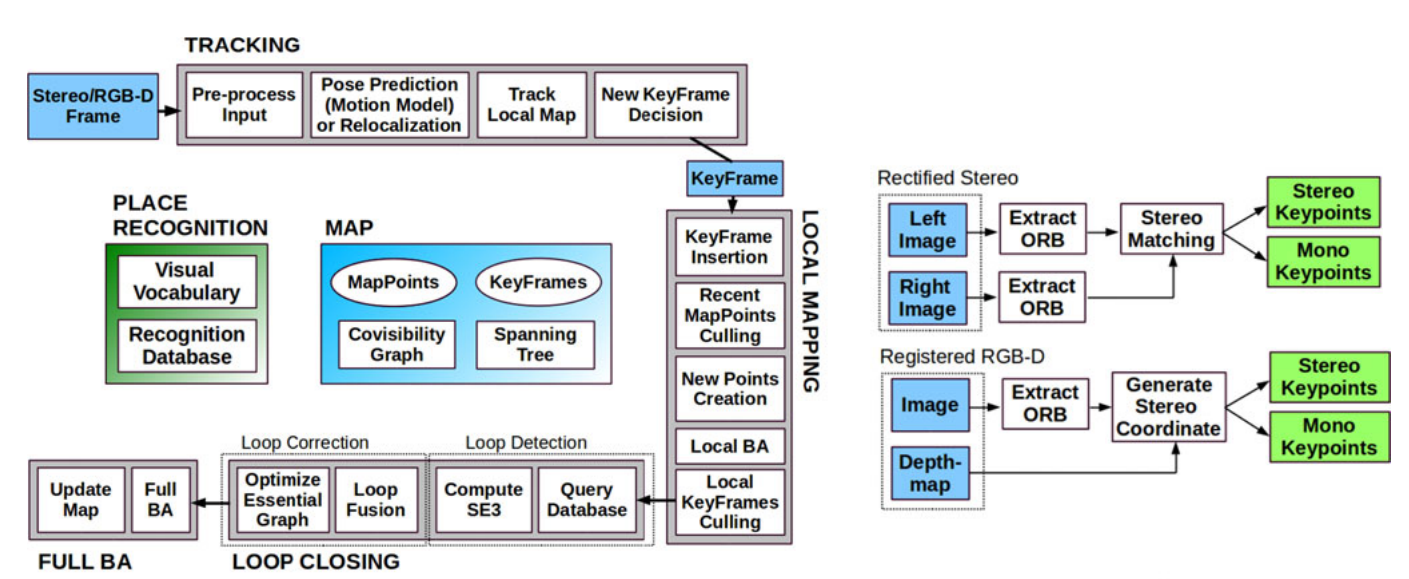
\includegraphics[width=300pt]{orb_framework.png}
  \caption{ORB-SLAM2的算法框架}
  \label{fig:orb_frame}
\end{figure}


\section{导航方案的迭代}

Tinker的开发过程中一直使用ROS作为主要开发框架,而ROS的Navigation Stack中对于
导航避障提供了一套较为成熟的解决方案。Tinker前后使用了2套定位与规划算法,下面两个
章节中将对这两套方案进行详细描述。

\subsubsection{路径规划与机器人控制}

ROS的Navigation stack中提供了一整套导航避障的解决方案。其核心是同时维护地图信息
与路径规划器。地图信息使用一种分层管理的方式\cite{lu2014layered},并且分别维护
全局地图 Global Map与局部地图 Local Map。规划器也有两个,分别是Global Planner
和Local Planner。其中 Global Planner负责根据全局地图生成路径,而 Local Planner
则负责根据局部地图生成速度指令,传输给底盘执行。Tinker使用的 Global Planner是
一种基于 Dijkstra算法\cite{deng2012fuzzy}的路径生成方法,Local Planner是
一种基于dynamic window approach的速度生成方案\cite{fox1997dynamic}。上述
方案均为机器人导航领域较为经典且通用的方案,Tinker团队对上述算法进行了一些微调,以
使算法在Tinker平台上有更好的表现,如图\ref{nav_costmap}所示为Tinker进行导航任
务时可视化的调试信息。

\begin{figure}[h] % use float package if you want it here
  \centering
  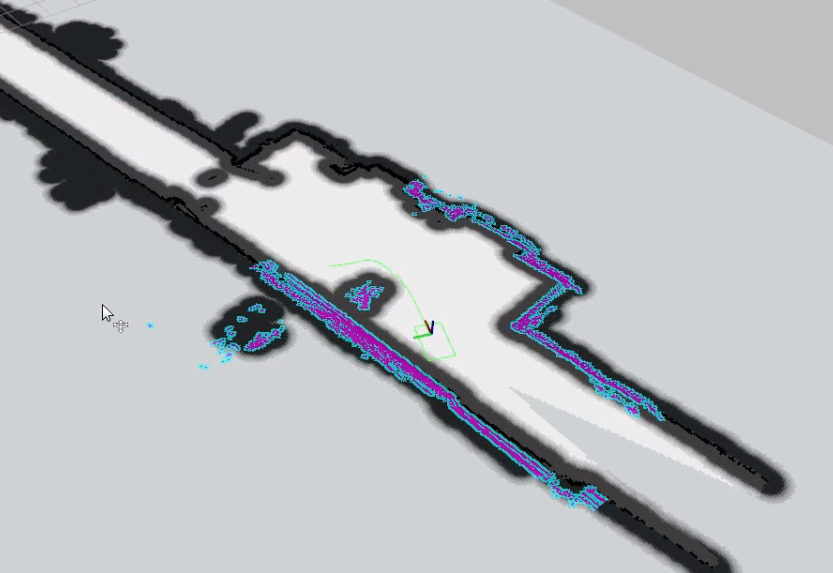
\includegraphics[width=300pt]{nav_costmap.png}
  \caption{进行导航任务时的地图与路径}
  \label{fig:nav_costmap}
\end{figure}


值得一提的是Tinker团队不断探索发现,在底盘接受速度命令端加一个smoother对临近的
几帧速度命令进行一定程度的加权平滑能够使机器人的运动性能得到质的提升。这一发现也提示
我们对于机器人这一复杂系统来说,提升整体性能的手段是多元的,在制定方案时应勇于尝试
多做实验,积极尝试各种想法,这样有助于我们使用较低的成本达到更好的性能。

